This section will elaborate on the steps we took to verify the results in the paper. The following steps were taken:

\begin{itemize}
	\item Generate graphs similar to the ones used in the paper.
	\item Implement the proposed algorithms to create optimized SQL queries from the graphs.
	\item Send query to SQL engine and measure the execution time
\end{itemize}

\noindent Figure~\ref{fig:process} gives an overview of the process and how the results are passed. The generation and translation of graphs are implemented in Java. The idea is to have a graph generator, which outputs the graph we want to solve. Specifically, we pass a list of graphs, which will be the graphs used for a single experiment, varying in graph order or density. \\

The graph translation part takes the graphs as input and generates SQL queries for the graphs, according to the algorithms proposed in the paper. This part thus returns several SQL queries, in a text-file and can be passed directly to the next part in the process. This is the biggest part of the assignment, so we want worked in parallel on the different algorithms. \\

The queries are passed to a SQL engine. We have chosen to use PostgreSQL, to stay close to the tools that were used in the paper. However, we no longer have access to the older version of Postgres that is used by the authors of the paper, so we choose to use a newer version, namely 9.3.4. The newer version can be more optimized, so we have to take this into account when comparing results. Furthermore, we know that the authors used a Linux cluster of Itanium II, processors with 4GB of memory. We have no access to the cluster and no further details about the hardware are available, so we have to use our own machines. The machine we will use has 32GB of RAM, but we are unsure whether our set-up, using an Intel Core i5-4670K (3.40 GHz), can match the computational power of the cluster. 

\begin{figure}
	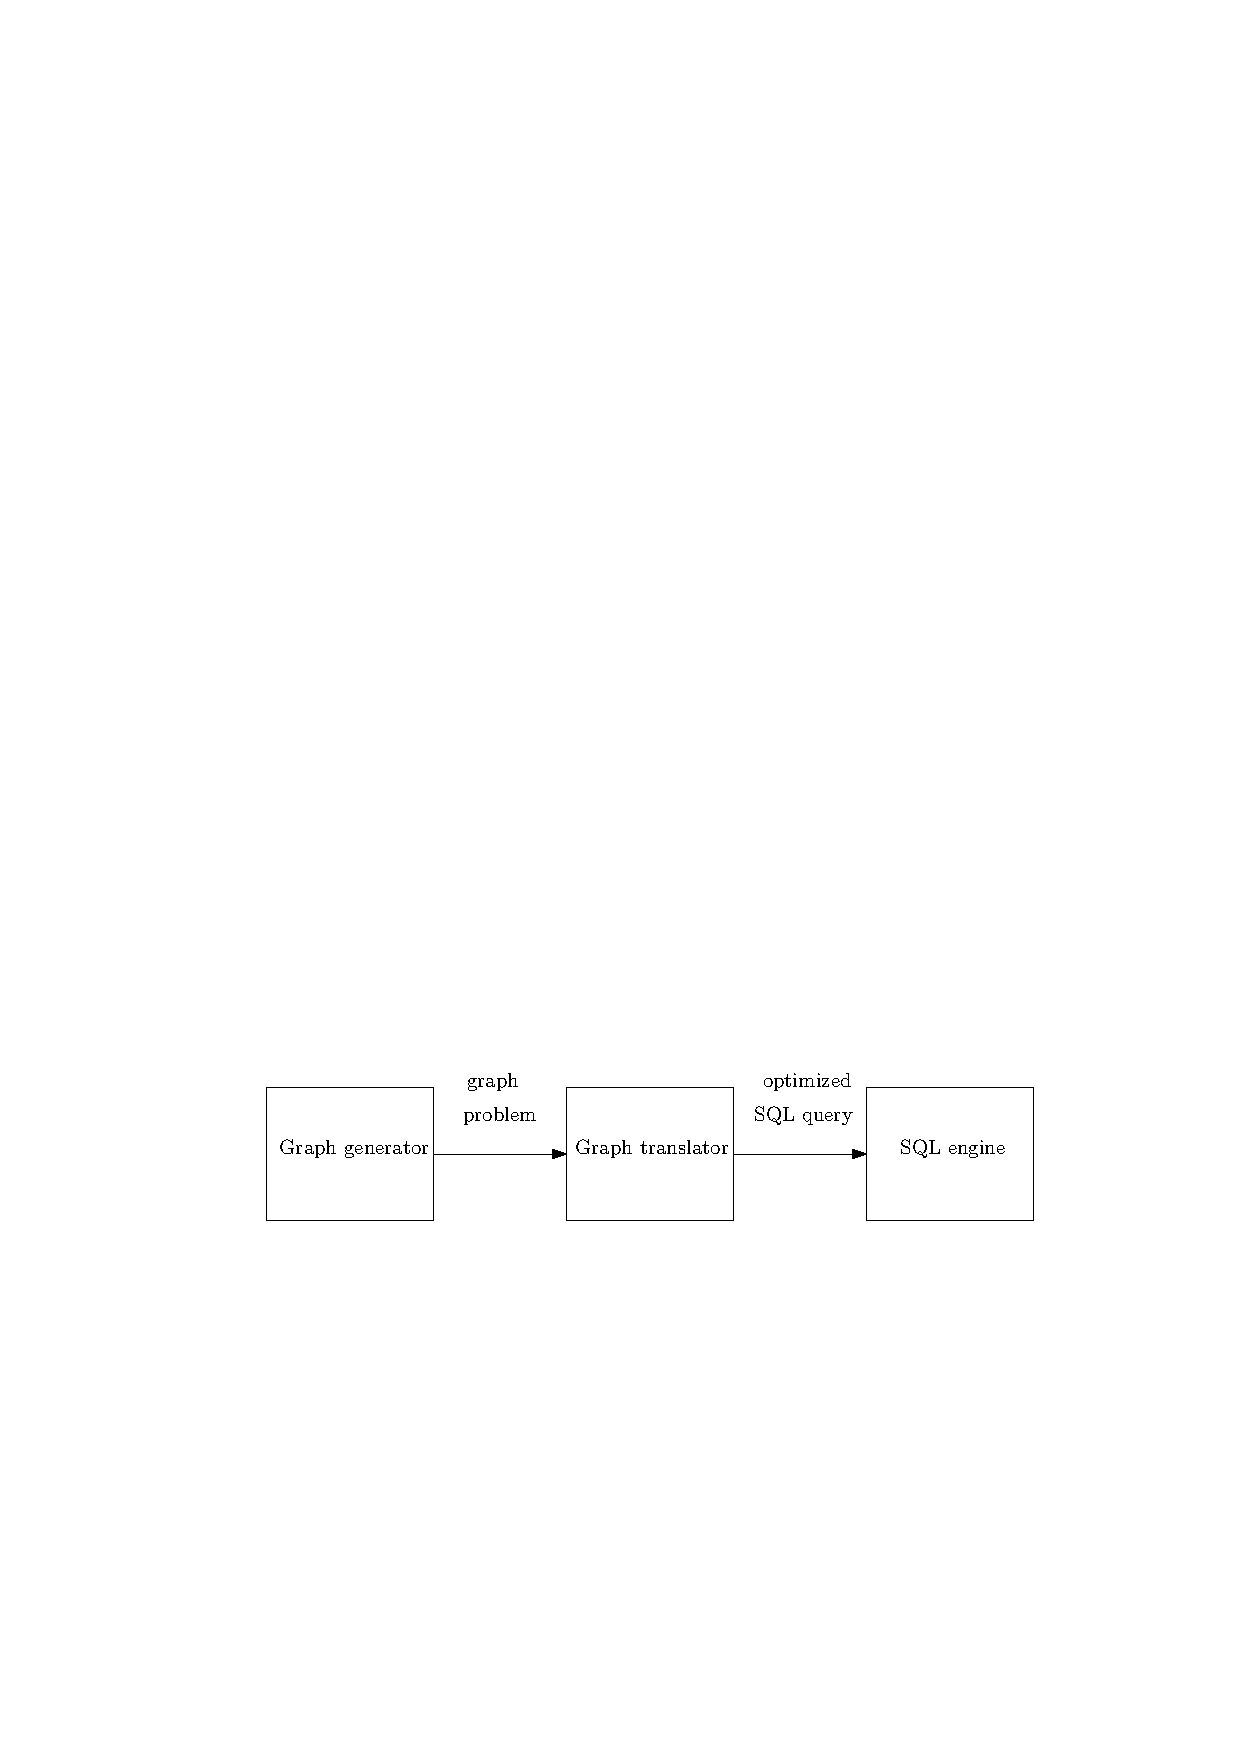
\includegraphics{figures/process.pdf}
	\caption{All steps in the process of verification}
	\label{fig:process}
\end{figure}

%TODO add for each step an detailed description